\setlength{\tabcolsep}{2pt}
\section{Experiments and Results}
\label{sec:results}

All our experiments have been completed with the inexpensive consumer
quadcopter called a Parrot's AR Drone 2.0. The imagery acquired were
from actual graffiti painted on large walls as well as posters in an
exhibition.  We have used the ROS-based ARDrone Autonomy
Driver to communicate with the drone. For the purpose of showing the
efficacy of our method, we also took a picture of the scene from a
distance with a smartphone camera to better understand the scene.

We have implemented our algorithm in C++ using the OpenCV library
(OpenCV 2.4.9). Experiments were performed on a PC with Intel Core i7
processor(@3.4GHz) and 8GB RAM.  
%The source code to produce
%interesting images from a video, and to generate the super-panorama,
%as well as the data sets used in this paper will be made publicly
%available after acceptance of the paper.

\subsection{Selecting Images}

In our first experiment, we wanted to ensure that the selection of
images done was comprehensive and useful.  We sent the drone to image 
an outdoor scene with no vacant space. This experiment was conducted
in an outdoor environment. We note here that there were approximately
3000 images in the raw video.  AutoStitch and Photoshop were unable to 
cope  when fed with this large number of frames.

One way to produce some sort of mosaic was to simply reduce the amount
of data given to AutoStitch.  Figure~\ref{fig:sac3}(a) shows uniformly
(time) sampled images from the video.  When these sampled images are
given to AutoStitch or to Adobe Photoshop, we find
(Figure~\ref{fig:sac3}(b)) that these programs are able to produce
some output, but the results are not satisfactory.

Instead of feeding time-sampled images, we ran our albumization
algorithm (as explained in Section~\ref{sec:selection}) on the video
which resulted in $N = 5$ images.  Though the number of input images
in the video is large, the total distance covered by the quadcopter in
this duration (of around 90 seconds) is small; thus the
number of distinct images returned by the algorithm shows a dramatic
reduction. Figure~\ref{fig:sac3}(c) shows examples of selected images.
Many of the images are similar to the time sampled version; however,
the occasional differences are enough to make AutoStitch work. The
results are shown in Figure~\ref{fig:sac3}(d).


\begin{figure}[hb!]
\centering
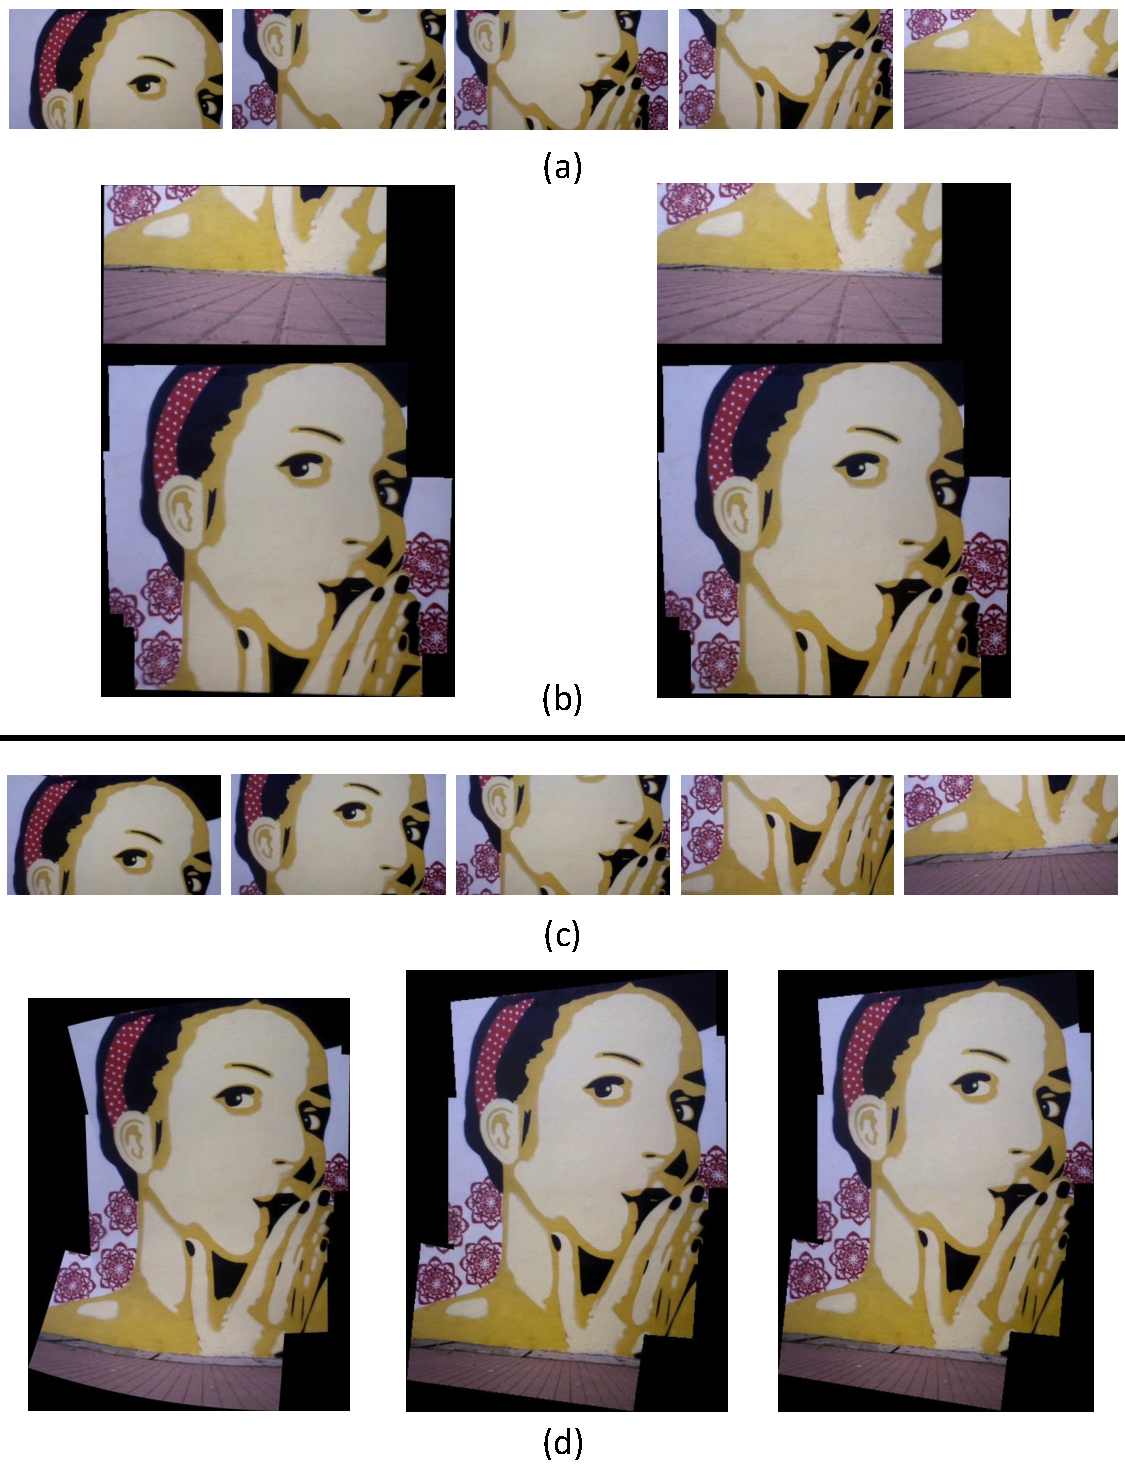
\includegraphics[width=0.87\linewidth]{figures/vacantSpaces/ValidationResult}
\caption[Validation Result: Lady]{ (a) Uniformly sampled images from an outdoor
video expedition.  (b) The output of the state of the art photo stitchers
  (left:AutoStitch, right:Adobe Photoshop CS6) on uniformly time
  sampled images.  As time sampled images do not guarantee coverage of
  the scene, the panorama is broken. The top portions do not belong at
  the right place (see (d)) (c) Salient image selection from the set of
  approximately 3000 images using positional information. (d) When
  salient images are given to AutoStitch (left) and Photoshop (middle),
  we can create a panoramic mosaic (since there are no vacant
  spaces). We also show the result from our stitching algorithm
  (bottom right).}
\label{fig:sac3}
\end{figure}

In summary, this experiment provides evidence to show that (a) our
albumization algorithm is reasonable and (b) our stitching
results are comparable to that of AutoStitch for the kind of scenes
considered.

\subsection{Indoor Imagery with Vacant Spaces}

Our next selection of experiments was conducted in an indoor
environment.  

The input stream had about 4300
images. The selection algorithm (Section~\ref{sec:selection}) pruned the video
into $N=5$ images. A sample of the selected images are seen in Figure~\ref{fig:vacantTeaser}.

There were two disconnected components in the resulting graph.
AutoStitch was unable to produce any reasonable output as seen in
Figure~\ref{fig:vacantTeaser}.  The scene, captured from a distance is also
shown.  One can see a better orthographic view of the posters.

\textbf{Cars:}
In an another experiment, the input stream had about 9000 input
images.  The selection algorithm (Section~\ref{sec:selection}) pruned
the video into $N=13$ images. A sample of the selected images are seen
in Figure~\ref{fig:indoor_results}(a).  The scene as captured by a
smartphone can also be seen, as well as the outputs of the state of
the art stitchers. Note that AutoStitch is only able to stitch the
upper half of the scene.  Our result
Figure~\ref{fig:indoor_results}(e) clearly stands out in comparison.

\begin{figure}
\centering
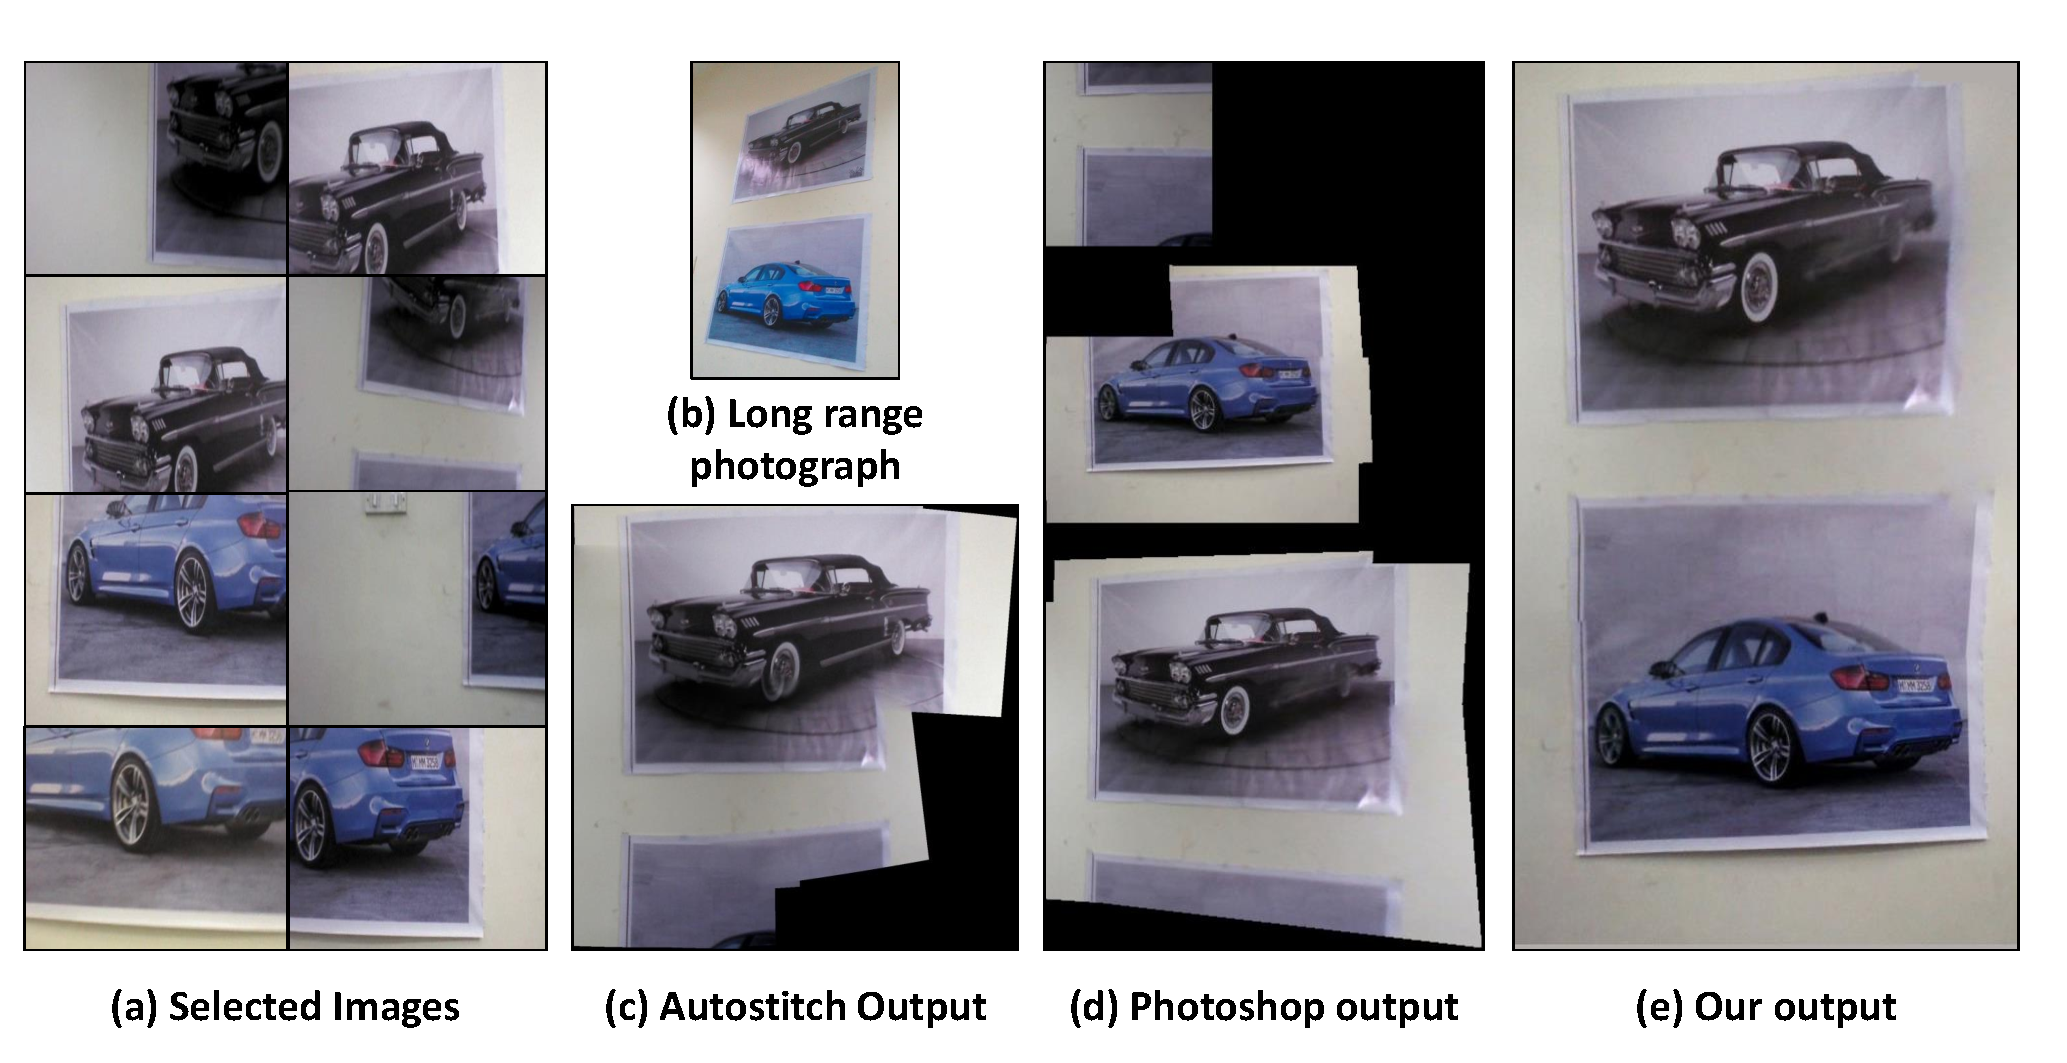
\includegraphics[width=\linewidth]{figures/vacantSpaces/indoor_results}
\caption[Result: Cars]{ (a) Pruned images from the quadcopter video using our
  saliency algorithm of (b) an indoor scene. This long range photograph
  has been captured separately by a smartphone camera only for
  context. Notice a significant vacant space in the imagery.  (c)
  The output of AutoStitch -- only the upper half of the scene is output.
  (d) The output of Adobe Photoshop CS6 -- the vacant space posed a problem to the
  feature matching algorithm, so instead of a mosaic, individual
  pieces were output as mini-panoramas (e) Our output on the selected
  images. We are able to present the scene in high fidelity in an
  orthographic view.}
\label{fig:indoor_results}
\end{figure}

\textbf{Aircrafts 1:} The input stream had about 9100 images. The selection
algorithm pruned the video into $N=14$ images. The scene as captured by a
smartphone can also be seen in Figure~\ref{fig:aircrafts1}(b). A sample of the
selected images is seen in Figure~\ref{fig:aircrafts1}(a).
Figure~\ref{fig:aircrafts1}(c,d,e) shows the comparison of outputs of state of
the art stitchers with the output of our algorithm. As there are vacant spaces,
AutoStitch~\cite{autostitch} is able to join only top part of the scene, while
Photoshop~\cite{photoshop} is showing two disconnected components.
In contrast, since we use positional data, our output is an acceptable mosaic,
and shows an orthographic view.

\begin{figure*}[h!]
	\centering
	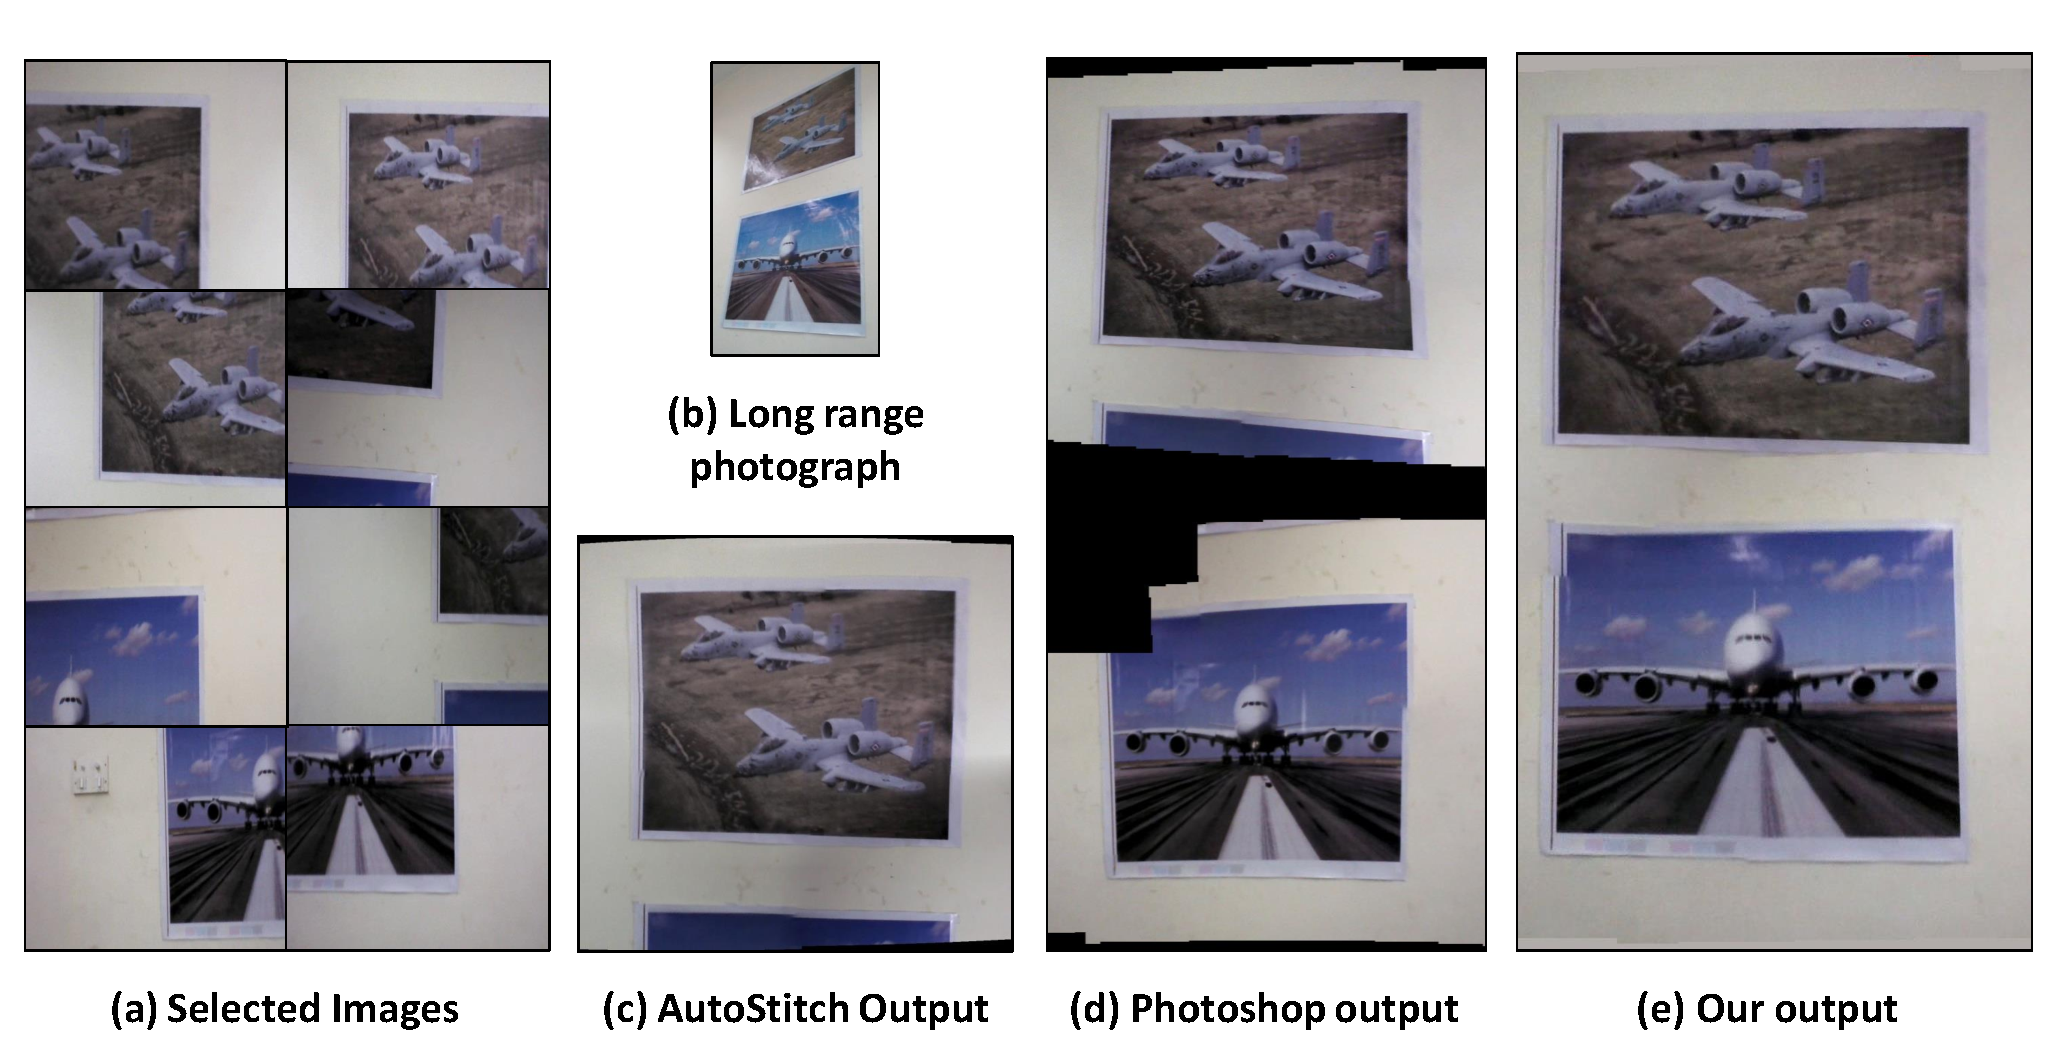
\includegraphics[width=\linewidth]{figures/vacantSpaces/aircrafts1}
	\caption[Result: Aircrafts]{(a) Pruned images from the quadcopter video using
	our saliency algorithm of (b) an indoor scene. This long range photograph has been captured separately by a smartphone camera only for context. Notice a significant vacant
space in the imagery. (c) The output of AutoStitch - only the upper half of the scene is output. (d) The output of Adobe Photoshop CS6 - 
the vacant space posed a problem to the feature matching algorithm, so instead of a mosaic, individual pieces were output as mini-panoramas (e) Our output on the
selected images. We are able to present the scene in high fidelity in an orthographic view.}
	\label{fig:aircrafts1}
\end{figure*}

\subsection{Outdoor Imagery with Vacant Spaces}

\begin{figure}[h!]
\centering
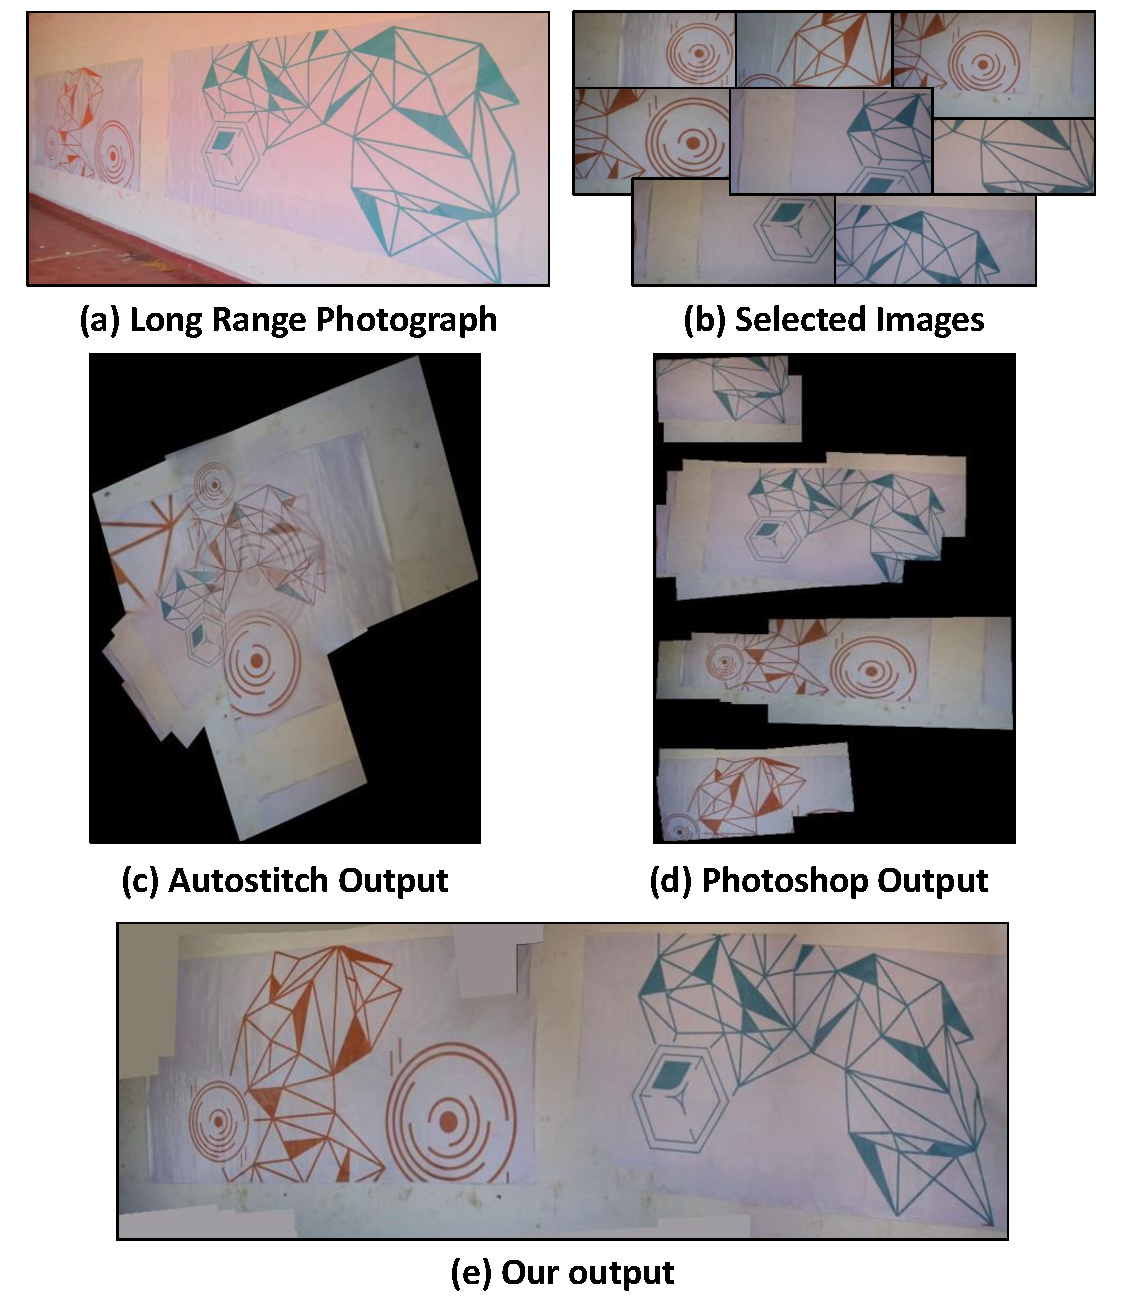
\includegraphics[width=\linewidth]{figures/vacantSpaces/orange_blue}
\caption[Result: Outdoor Exhibition]{(a) An outdoor scene captured by a standard
camera in an exhibition. The approach to the area is normally cordoned off and one
  needs permission to get a quadcopter to take the picture.  Notice a
  significant gap between the two posters.  (b) Pruned images from the
  quadcopter video using our saliency algorithm. (c) The output of
  AutoStitch on the selected images. The mosaic is not reasonable
  presumably because of the confusion in features. (d) The output of Adobe
  Photoshop CS6 on the selected images. The vacant space posed a
  problem to the feature matching algorithm, so instead of a mosaic,
  individual pieces were output as mini-panoramas (e) Our output on
  the selected images. We are able to join two posters (separated by
  vacant space) using the IMU data.}
\label{fig:results}
\end{figure}

Our next set of experiments were conducted in an outdoor
environment. The input stream had about 12000 images. The selection
algorithm pruned the video into $N=30$ images. A sample of the
selected images are seen in Figure~\ref{fig:results}(a).  The scene as
captured by a smartphone can be seen in Figure~\ref{fig:results}(b).
Figures~\ref{fig:results}(c), (d) and (e) shows the comparison of outputs of
state of the art stitchers with the output of our algorithm. Note that
AutoStitch is getting confused by too many matching features. 
Please see supplementary material for results on other indoor as well as outdoor datasets.

Figure \ref{fig:results2} shows comparison of outputs of state of the art
stitchers with the output of our algorithm on another dataset.

\begin{figure}[h!]
\centering
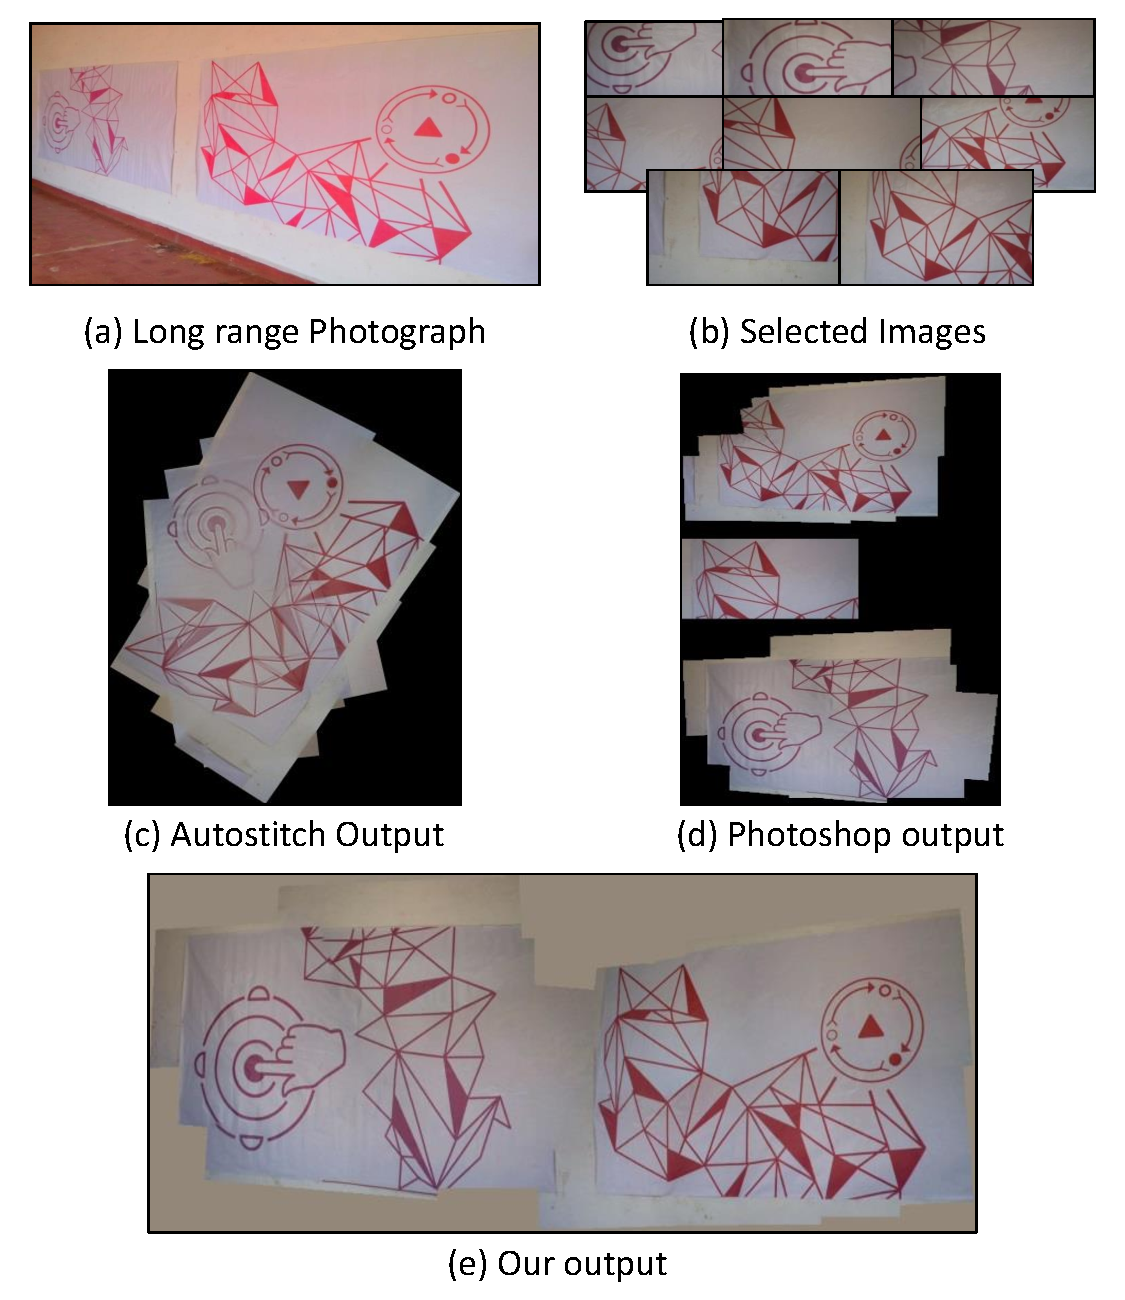
\includegraphics[width=\linewidth]{figures/vacantSpaces/Purple_red} 
\caption[Result: Outdoor
Exhibition 2]{(a) Another outdoor
scene captured by a standard camera in an exhibition. The approach to the area is normally cordoned off and one
  needs permission to get a quadcopter to take the picture.  Notice a
  significant gap between the two posters.  (b) Pruned images from the
  quadcopter video using our saliency algorithm. (c) The output of
  AutoStitch on the selected images. The mosaic is not reasonable
  presumably because of the confusion in features. (d) The output of Adobe
  Photoshop CS6 on the selected images. The vacant space posed a
  problem to the feature matching algorithm, so instead of a mosaic,
  individual pieces were output as mini-panoramas (e) Our output on
  the selected images. We are able to join two posters (separated by
  vacant space) using IMU data.}
\label{fig:results2}
\end{figure}


\subsection{Analysis}

The performance of our algorithm as a function of the scene, as well
comparison with other software is summarized in
Table~\ref{tbl:results}.  It can be seen that, whenever there is
vacant space between adjacent images, AutoStitch produces only
one component, presumably the largest.  Adobe Photoshop outputs all disconnected
components. Sometimes due to the lack of spatial proximity
information, the resulting images (or components) are disconnected instead of being 
mosaiced (unlike AutoStitch). In contrast, in all cases, our algorithm
successfully uses proximity information which results in a reduced number of mini-panoramas. 

As expected the number of selected images in our saliency algorithm
varies based on environment considerations (outdoor/indoor), the
average depth from the scene, and the total scene area.
 
\begin{table*}
\scriptsize

\newcolumntype{C}{ >{\centering\arraybackslash} m{1.1cm} }
\newcolumntype{D}{ >{\centering\arraybackslash} m{1.5cm} }

\begin{tabular}{|C|C|C|C|D|D|D|m{6.5cm}|}
\hline
Dataset 
& Number of Images in video 
& Approx. planar area covered
& Number of selected images 
& AutoStitch: \# Components 
& Photoshop: \# Components
& Our algorithm: \#mini- panoramas
& \multicolumn{1}{p{6.5cm}|}{\centering Remarks}\\
\hline

\hyperref[fig:sac3]{Lady} & 3000 & 60 sqft. & 5 & 1 & 1 & 1 & As there are enough features
in the intersection of selected images, AutoStitch, Photoshop as well
as our algorithm produces the  panorama correctly.\\\hline
%Spray Woman} & 9000 & 70 sqft. & 15 & 1 &
%1 & 1 & As there are enough features in the intersection of selected images,
%AutoStitch, Photoshop as well as our algorithm gives full panorama
%correctly. As this scene was captured nearer from the plane than
%earlier, we need to select more images than earlier dataset.\\\hline 

\hyperref[fig:vacantTeaser]{Indoor exhibition} & 4300 & 40 sqft. & 5 &
1 & 2 & 2 & As there is vacant space between the two posters,
AutoStitch produces only one panoramic image. Photoshop outputs two
posters as two disconnected components; these correspond to our mini-panoramas.
\\\hline 

\hyperref[fig:indoor_results]{Cars} & 9000 & 60 sqft. & 13 & 1 & 3 & 3 &
As there is vacant space between the two visuals, AutoStitch produces
only one panoramic image, the black vehicle.  In the case of
Photoshop, two of the three disconnected 
components represents two partial visuals, while the third component is
the intersection  between the two cars -- this portion contains featureless
space.\\\hline

\hyperref[fig:results]{Outdoor exhibition} & 12000 & 80 sqft. &
30 & 1 & 4 & 2 &  AutoStitch is confused by the replicated features in
the two posters which are sometimes proximal and sometimes
geographically distant.  A single panorama is produced, but the output
is incorrect. We use the IMU data
for arranging the images in a spatial neighborhood; we have fewer
mini-panoramas.  Photoshop is not able to produce a super-panorama and
the number of disconnected components in Photoshop's output is larger
than the number of mini-panoramas.\\\hline  
\end{tabular}
\caption{Quantitative summary of  results}
\label{tbl:results}
\end{table*}

